\documentclass[11pt,letterpaper]{article}
\usepackage[top=3cm, bottom=2cm, left=2cm, right=2cm, columnsep=20pt]{geometry}
\usepackage{pdfpages}
\usepackage{graphicx}
\usepackage{etoolbox}
\apptocmd{\sloppy}{\hbadness 10000\relax}{}{}
% \usepackage[numbers]{natbib}
\usepackage[T1]{fontenc}
\usepackage{ragged2e}
\usepackage[french]{babel}
\usepackage{listings}
\usepackage{color}
\usepackage{soul}
\usepackage[utf8]{inputenc}
\usepackage[export]{adjustbox}
\usepackage{caption}
\usepackage{amsmath}
\usepackage{amssymb}
\usepackage{float}
\usepackage{csquotes}
\usepackage{fancyhdr}
\usepackage{wallpaper}
\usepackage{siunitx}
\usepackage[indent]{parskip}
\usepackage{textcomp}
\usepackage{gensymb}
\usepackage{multirow}
\usepackage[hidelinks]{hyperref}
\usepackage{abstract}
\renewcommand{\abstractnamefont}{\normalfont\bfseries}
\renewcommand{\abstracttextfont}{\normalfont\itshape}
\usepackage{titlesec}
\titleformat{\section}{\large\bfseries}{\thesection}{1em}{}
\titleformat{\subsection}{\normalsize\bfseries}{\thesubsection}{1em}{}
\titleformat{\subsubsection}{\normalsize\bfseries}{\thesubsubsection}{1em}{}

\usepackage{xcolor}
\definecolor{codegreen}{rgb}{0,0.6,0}
\definecolor{codegray}{rgb}{0.5,0.5,0.5}
\definecolor{codepurple}{rgb}{0.58,0,0.82}
\definecolor{backcolour}{rgb}{0.95,0.95,0.92}
\lstdefinestyle{mystyle}{
    backgroundcolor=\color{backcolour},   
    commentstyle=\color{codegreen},
    keywordstyle=\color{magenta},
    numberstyle=\tiny\color{codegray},
    stringstyle=\color{codepurple},
    basicstyle=\ttfamily\footnotesize,
    breakatwhitespace=false,         
    breaklines=true,                 
    captionpos=b,                    
    keepspaces=true,                 
    numbers=left,                    
    numbersep=5pt,                  
    showspaces=false,                
    showstringspaces=false,
    showtabs=false,                  
    tabsize=2
}
\lstset{style=mystyle}

\usepackage[most]{tcolorbox}
\newtcolorbox{note}[1][]{
  enhanced jigsaw,
  borderline west={2pt}{0pt}{black},
  sharp corners,
  boxrule=0pt, 
  fonttitle={\large\bfseries},
  coltitle={black},
  title={Note:\ },
  attach title to upper,
  #1
}

%----------------------------------------------------

\setlength{\parindent}{0pt}
\DeclareCaptionLabelFormat{mycaptionlabel}{#1 #2}
\captionsetup[figure]{labelsep=colon}
\captionsetup{labelformat=mycaptionlabel}
\captionsetup[figure]{name={Figure }}
\newcommand{\inlinecode}{\normalfont\texttt}
\usepackage{enumitem}
\setlist[itemize]{label=\textbullet}

\begin{document}
\begin{titlepage}
\center

\begin{figure}
    \ThisULCornerWallPaper{.4}{Polytechnique_signature-RGB-gauche_FR.png}
\end{figure}
\vspace*{2 cm}

\textsc{\Large \textbf{PHS2223 --} Introduction à l'optique moderne}\\[0.5cm]
\large{\textbf{Équipe : 04}}\\[1.5cm]

\rule{\linewidth}{0.5mm} \\[0.5cm]
\Large{\textbf{Expérience 4}} \\[0.2cm]
\text{Filtrage spatial}\\
\rule{\linewidth}{0.2mm} \\[2.3cm]

\large{\textbf{Présenté à}\\
  Guillaume Sheehy\\
  Esmat Zamani\\[2.5cm]
  \textbf{Par :}\\
  Émile \textbf{Guertin-Picard} (2208363)\\
  Laura-Li \textbf{Gilbert} (2204234)\\
  Tom \textbf{Dessauvages} (2133573)\\[3cm]}

\large{\today\\
Département de Génie Physique\\
Polytechnique Montréal\\}

\end{titlepage}

%----------------------------------------------------

\tableofcontents
\pagenumbering{roman}
\newpage

\pagestyle{fancy}
\setlength{\headheight}{14pt}
\renewcommand{\headrulewidth}{0pt}
\fancyfoot[R]{\thepage}

\pagestyle{fancy}
\fancyhf{}
\renewcommand{\headrulewidth}{1pt}
\fancyhead[L]{\textbf{PHS2223}}
\fancyhead[C]{Rapport préliminaire}
\fancyhead[R]{\today}
\fancyfoot[R]{\thepage}

\pagenumbering{arabic}
\setcounter{page}{1}

%----------------------------------------------------

\section{Introduction}

\section{Théorie}
Afin de comprendre les différents phénomènes physiques réalisés lors de cette expérience, cette section présente les principes physiques et mathématiques importants relativement à l'expérimentation.

\subsection{Optique de Fourier}\label{Fourier_optic}
L'optique de Fourier, principalement basée sur les idées de convolution, de corrélation spatiale et de transformée de Fourier, est une approche mathématique utilisée pour décrire et analyser la propagation d'ondes lumineuses. Cette méthode considère, contrairement à l'optique géométrique, la nature ondulatoire de la lumière, ainsi la forme de l'onde consiste en une combinaison, ou une superposition, d'ondes planes et, plus précisément, d'ondes sphériques \textcolor{red}{(Source 1)}. De cette manière, en plus de la trajectoire de la lumière, l'optique de Fourier permet d'étudier les variations d'amplitude et de phase causées par les phénomènes d'interférence et de diffraction. En appliquant la transformée de Fourier sur les ondes lumineuses, donnée par la formule suivante :
\begin{equation}
  \mathcal{F}(k)=\int_{-\infty}^{\infty}f(x)e^{-ikx}dx
\end{equation}
Il est possible de décomposer un champ optique en somme de fréquence spatiales, chacune correspondant à une direction et à une propagation spécifique \textcolor{red}{(Source 2)}. L'optique de Fourier est, généralement, utilisée pour la lumière monochromatique, décrite  par des amplitudes complexes, et pour un modèle d'onde purement scalaire. Mathématiquement, cette notion se transcrit en commençant avec l'équation d'onde homogène donnée par :
\begin{equation}
  \left(\nabla^{2}-\frac{1}{c^{2}}\frac{\partial^{2}}{\partial t^{2}}\right)u(\mathbf{r}, t)=0
\end{equation}
Où $u(\mathbf{r}, t)$ est une fonction d'onde scalaire. En d'autres termes, en considérant une onde lumineuse de fréquence fixe, tel qu'un laser monomode, il est possible d'assumer, à l'aide de la dépendance temporelle des solutions d'onde à la fréquence angulaire, que la fonction d'onde scalaire est donnée par :
\begin{equation}
  u(\mathbf{r}, t)=\mathrm{Re}\{\psi(\mathbf{r})e^{i\omega t}\}
\end{equation}
À partir de ces équations ci-dessus et sous certaines conditions, telles que $z$ est nul, il est possible d'obtenir une solution générale, pour une fréquence fixe, à l'équation d'ondes homogène, soit une intégrale de la superposition de l'ensemble des solutions d'ondes planes \textcolor{red}{(Source 3)}.
\begin{equation}
  \psi(x, y, z)=\int_{-\infty}^{\infty}\int_{-\infty}^{\infty}\Psi_{0}(k_{x},k_{y})e^{i(k_{x}x+k_{y}y)}dk_{x}dk_{y}
\end{equation}
Correspondant simplement à une relation de transformée de Fourier entre le champ et les composantes de l'ondes. Ainsi, la transformation de Fourier permet de passer de la description spatiale d’un champ lumineux à sa description dans le domaine fréquentiel.

% Source 1 : https://www.rp-photonics.com/fourier_optics.html
% Source 2 : https://www.sciencedirect.com/topics/physics-and-astronomy/fourier-optics
% Source 3 : https://en.wikipedia.org/wiki/Fourier_optics

\subsection{Diffraction}
La diffraction est un phénomène physique correspondant à une interférence, ou une diffusion, des ondes autour des points d'une ouverture \textcolor{red}{(Source A)}. En optique, deux types de diffraction peuvent être observés : la diffraction de Fresnel et la diffraction de Fraunholer. Dans le cas de Fresnel, ce type de diffraction survient lorsque la source, ou le plan image, est relativement près de le l'ouverture, c'est-à-dire en champ proche. La diffraction de Fraunholer, pour sa part, se produit lorsque la source de lumière et le plan image sont suffisamment distancés de l'objet afin que les ondes puissent être considérées comme parallèles \textcolor{red}{(Source B)}.

% Source A : https://www.olympus-lifescience.com/fr/microscope-resource/primer/lightandcolor/diffraction/
% Source B : pdf FourierOptics

\subsubsection{Approximation de Fraunholer}
L'approximation de Fraunholer correspond à une simplification mathématique de la diffraction pour les champs lointains. Cette approximation permet d'analyser les patrons de diffraction produits par les objets diffractants, en décrivant les ondes lumineuses comme planes après le passage de l'objet. Mathématiquement, cette approximation peut se traduire de la manière suivante :
\begin{equation}
  U(x,y,z)=\int_{-\infty}^{\infty}\int_{-\infty}^{\infty}A(x',y')e^{-i(f_{x}x'+f_{y}y')}dx'dy'
\end{equation}
En optique, cette équation, l'équation de diffraction de Fraunholer, est utilisée afin d'obtenir directement le motif de diffraction en fonction de sa transformée de Fourier \textcolor{red}{(Source C)}. 

% Source C : https://phys.libretexts.org/Bookshelves/Optics/BSc_Optics_(Konijnenberg_Adam_and_Urbach)/06%3A_Scalar_diffraction_optics/6.07%3A_Fresnel_and_Fraunhofer_Approximations

\subsection{Système 4F}
Les systèmes optiques à configuration 4F sont des systèmes utilisant l'optique de Fourier. Ces systèmes de deux lentilles sont couramment utilisés pour manipuler les fréquences spatiales d'une image en exploitant la transformée de Fourier des objets des plans focaux. La configuration 4F comprend un plan objet, situé à une distance de la première lentille égale à la focale de cette dite lentille, et un plan image, situé à une distance focale derrière la seconde lentille. Les deux lentilles sont séparées par le plan de Fourier, où l'objet subit une transformée de Fourier \textcolor{red}{(Source Alpha)}.

Le fonctionnement de ce type de configuration repose sur le principe de la transformée de Fourier. En effet, la première lentille transforme l'objet en une image de Fourier, c'est-à-dire que celle-ci est décomposée en composante de fréquence spatiale. Dans le plan de Fourier, où il est possible d'ajouter des filtres optiques, l'image transmise par la première lentille subit une transformée de Fourier. Cette transformée est, ensuite, transmise à la seconde lentille qui, par la transformée inverse, reconstitue l'image de l'objet. Cette image est, finalement, transmise au plan image afin d'être observée \textcolor{red}{(Source Bravo)}.

% Source Alpha : https://www.opticsforhire.com/blog/4f-optical-system-fourier-optics/

% Source Bravo : pdf nikhef

\subsection{Signaux, images et filtres}
Tel que mentionné dans la section \ref{Fourier_optic}, l'optique de Fourier permet de passer au domaine fréquentiel spatial. De cette manière, les signaux, en optique de Fourier, correspondent à des distributions d'intensité lumineuses, ou phasiques, en fonction de la fréquence spatiale. Les images, produites par le traitement des signaux, sont alors représentées en termes de ces fréquences spatiales.

Avec cette notion spatiale, les filtres, permettant la sélection de certaines composantes spatiales, peuvent être utilisés afin de manipuler l'information fréquentielle contenue dans les images, que ce soit en atténuant le bruit, en choisissant certaines fréquences, ou en accentuant les bords \textcolor{red}{(Source Z)}. Les filtres utilisés peuvent être de trois types différents : passe-bas, passe-haut et passe-bande. Par exemple, dans l'expérience réalisée, un filtre passe-bas haut-de-forme est utilisé, c'est-à-dire que les seules fréquences pouvant passer sont les basses fréquences spatiales jusqu'à une certaine coupure. Un autre filtre utilisé est le filtre gaussien qui, dans son cas, permet d'atténuer progressivement les hautes fréquences spatiales suivant une distribution gaussienne.

% Source Z : https://fiveable.me/optical-computing/unit-4/fourier-optics-spatial-filtering/study-guide/cGhLAP7EssS8bwjb

\section{Méthodologie}

\subsection{Présentations des montages}

\subsection{Explications}

\section{Hypothèses}

Afin de mieux comprendre et prédire ce qui sera vu avec les montages présentés précédemment, il est possible d'émettre quelques hypothèses en lien avec l'application de filtres sur des images. Cette section présente donc le filtrage et l'analyse d'images de référence disponible dans le répertoire du cours.

\subsection{Patron d'échec}

La première image filtrée est un simple patron d'échec. Pour appliquer un filtre, la transformée de Fourier de l'image est prise, tel qu'affiché à la figure \ref{echec_patron} :

\begin{figure}[H]
  \centering
  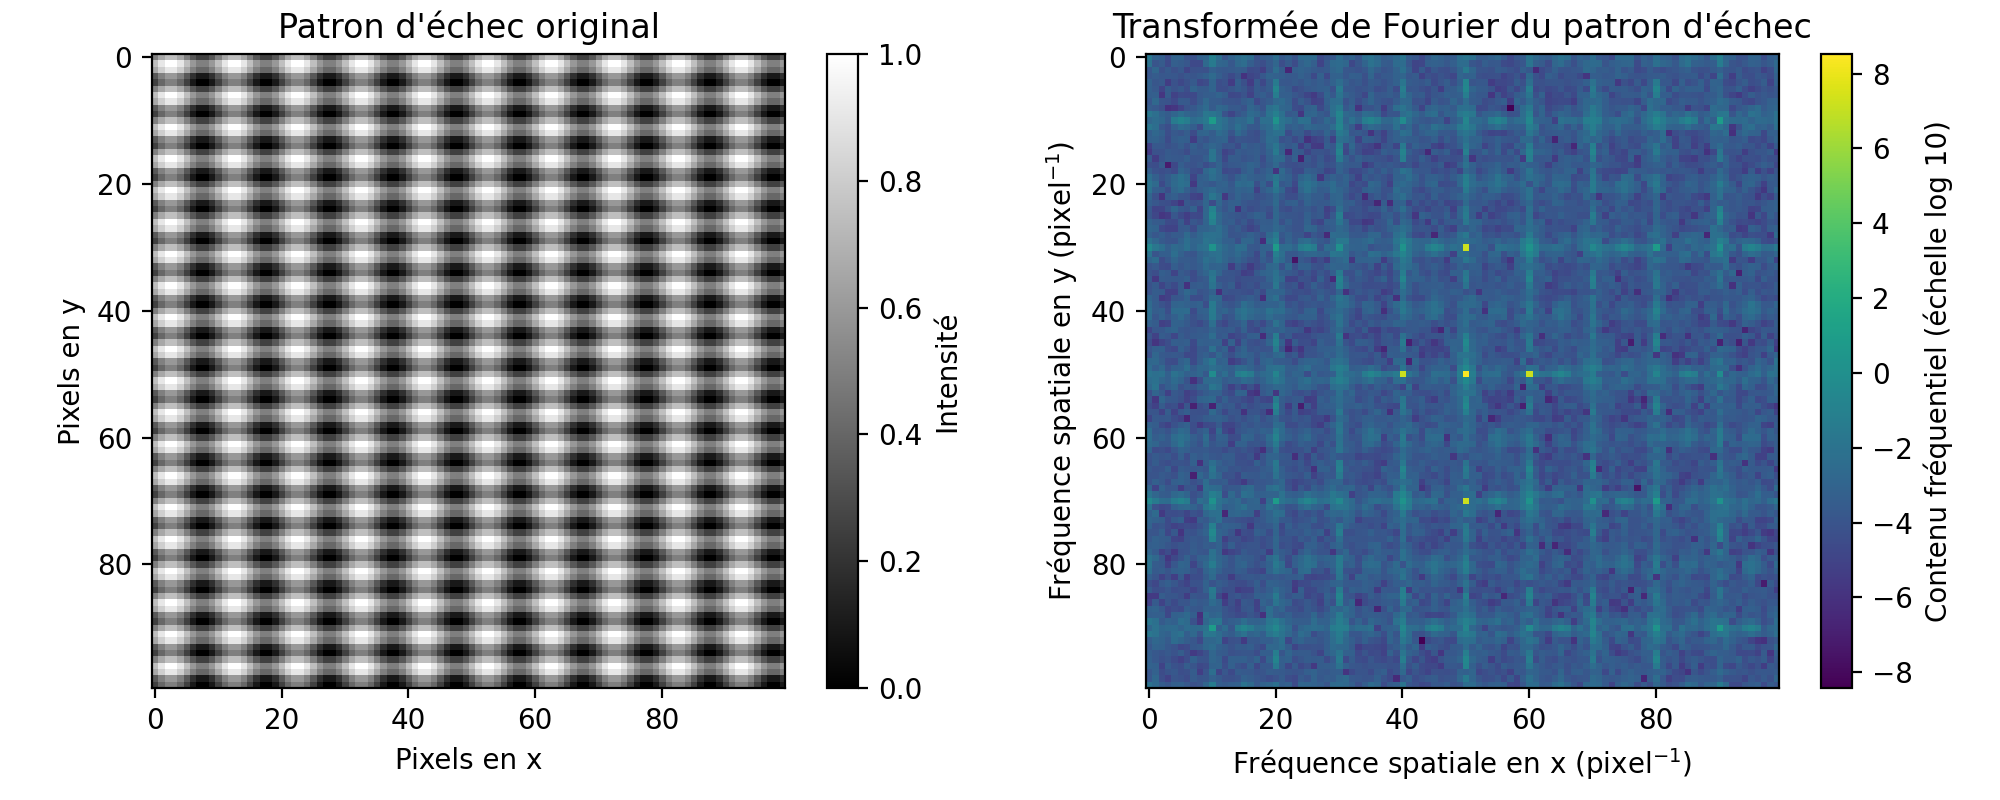
\includegraphics[scale=0.68]{check.png}
  \caption{Affichage du patron d'échec original et de sa transformée de fourier}
  \label{echec_patron}
\end{figure}

Pour enlever les oscillations en $\hat{y}$, la fonction fenêtre de la figure \ref{echec_filtre}, qui agit comme filtre passe-bande, est appliquée sur la transformée de Fourier :

\begin{figure}[H]
  \centering
  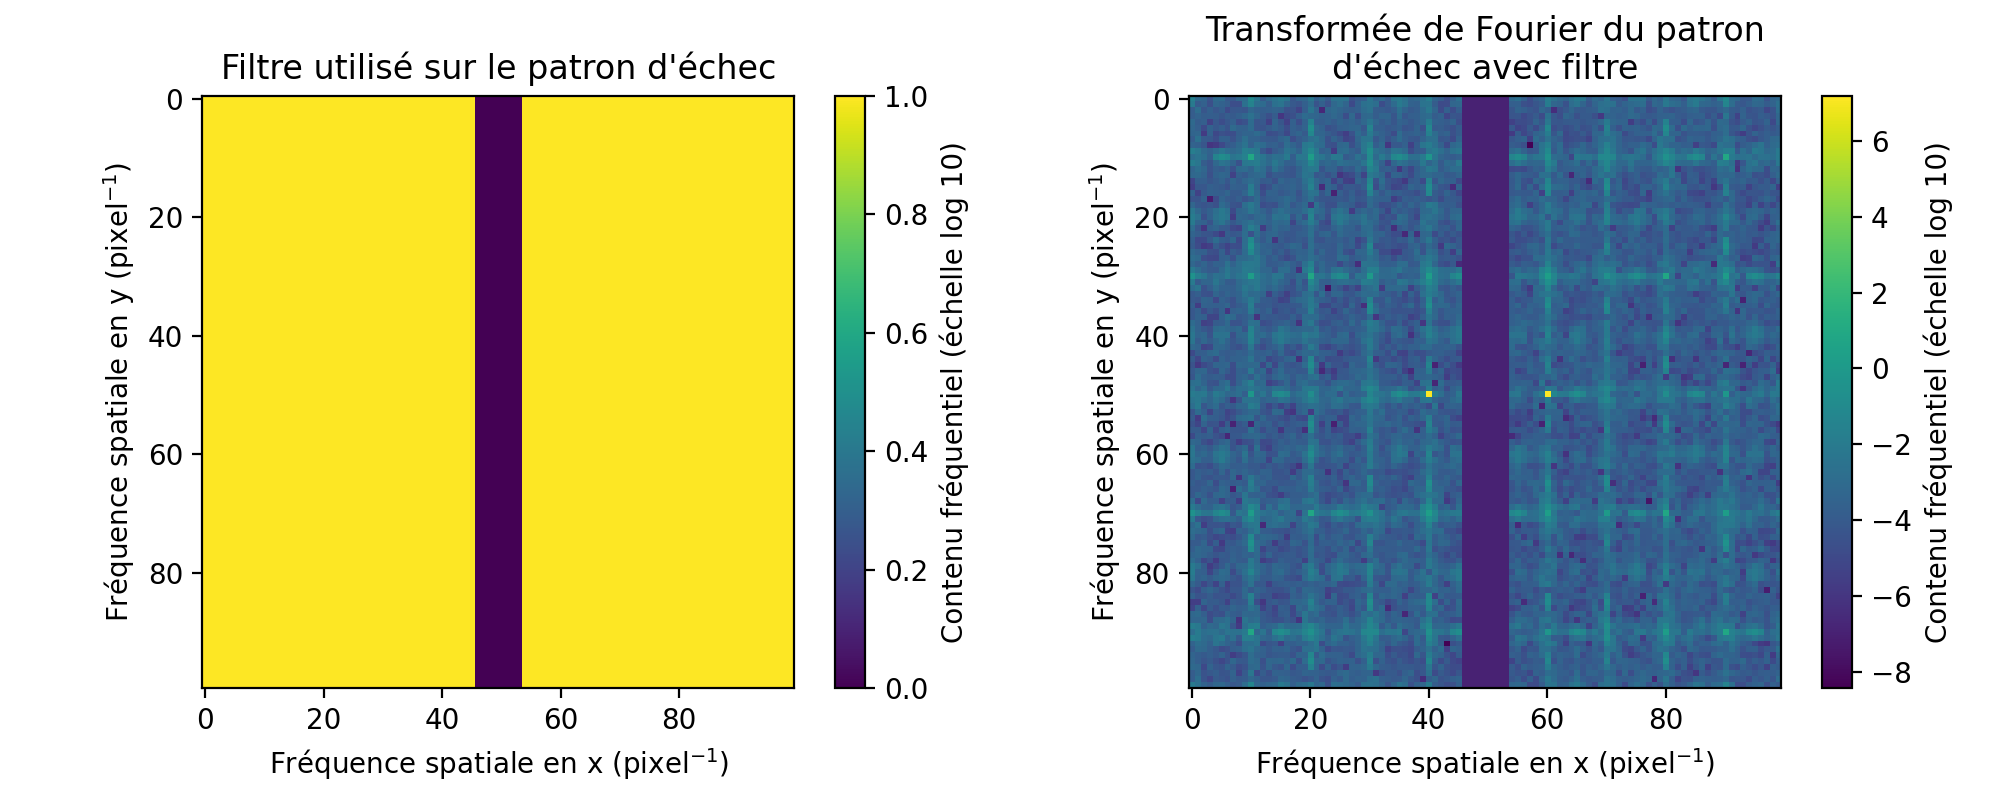
\includegraphics[scale=0.68]{check_mask.png}
  \caption{Filtre utilisé pour enlever les oscillations en $\hat{y}$ et son applications sur la transformée de Fourier}
  \label{echec_filtre}
\end{figure}

Enfin, la transformée inverse sur l'application du filtre donne le patron d'échec avec toutes les orcillations en $\hat{y}$ filtrées, tel que montré à la figure \ref{echec_comp} :

\begin{figure}[H]
  \centering
  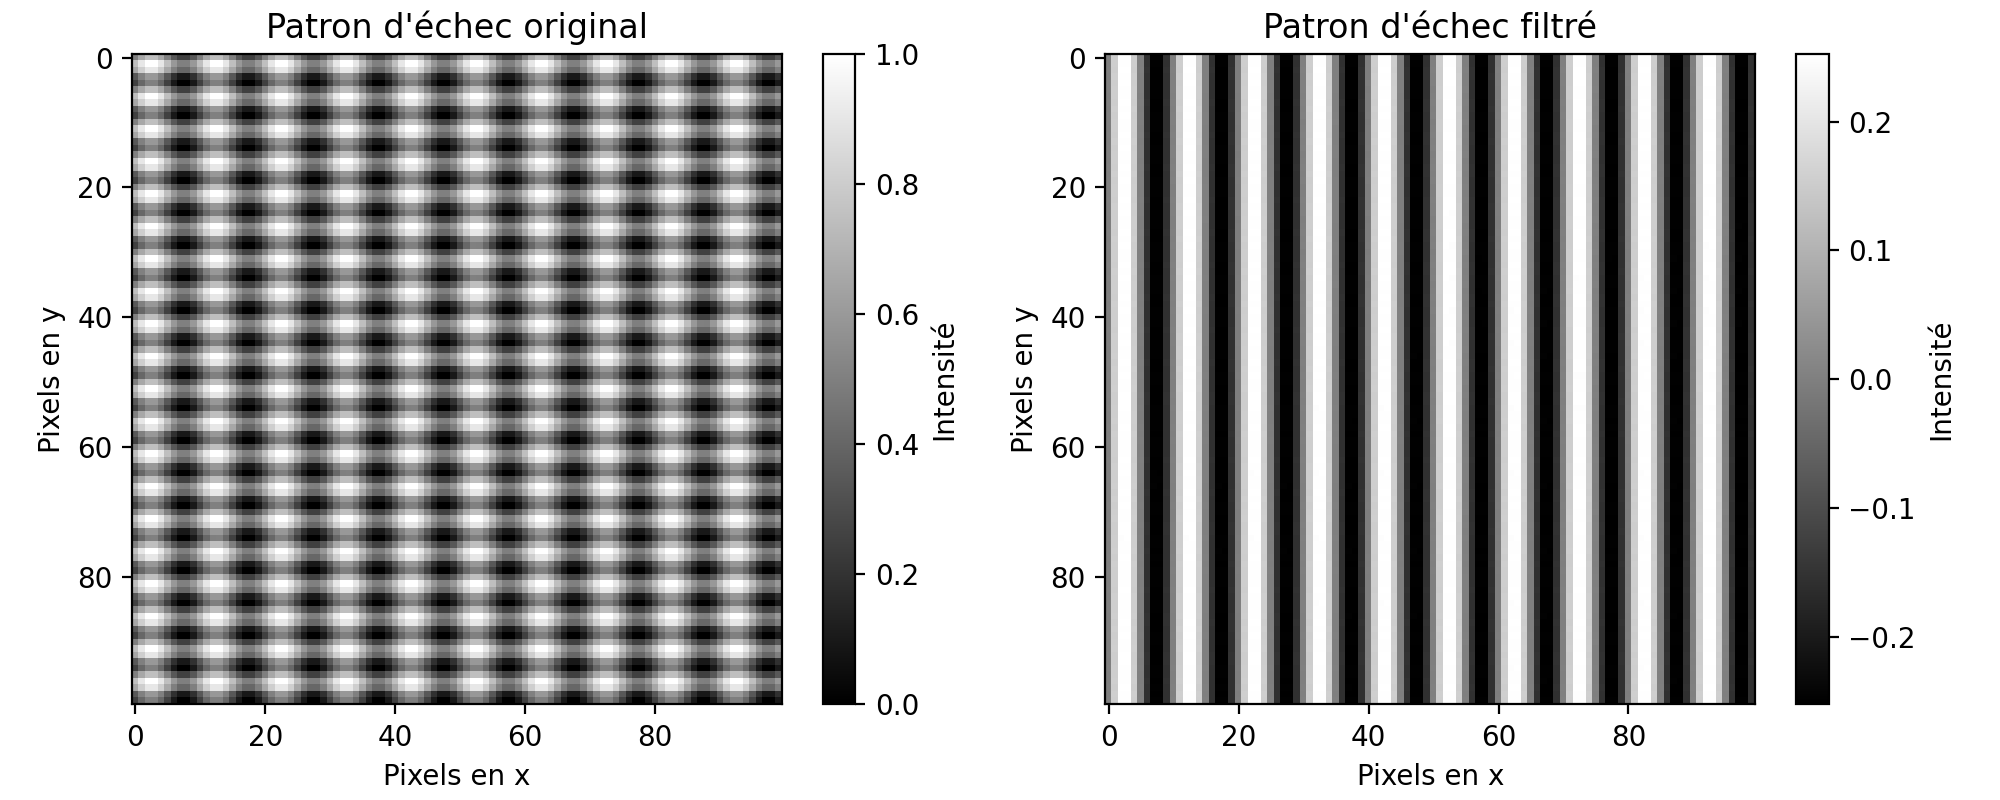
\includegraphics[scale=0.68]{check_filtre.png}
  \caption{Comparaison entre le patron d'échec initial et filtré}
  \label{echec_comp}
\end{figure}

\subsection{Filtres passe-bas top-hat}

La seconde image filtrée est celle du chat Marvin. Il est possible de la voir ainsi que sa transformée de Fourier à la figure \ref{cat_og}. Ensuite, des filtre passe-bas top hat sont défini aussi comme des fenêtres mais circulaires. Il est possible de voir ces filtres et leurs applications aux figures \ref{fc50hat}, \ref{fc75} et \ref{fc100} pour $f_c = 50, 75,100$ respectivement.

\begin{figure}[H]
  \centering
  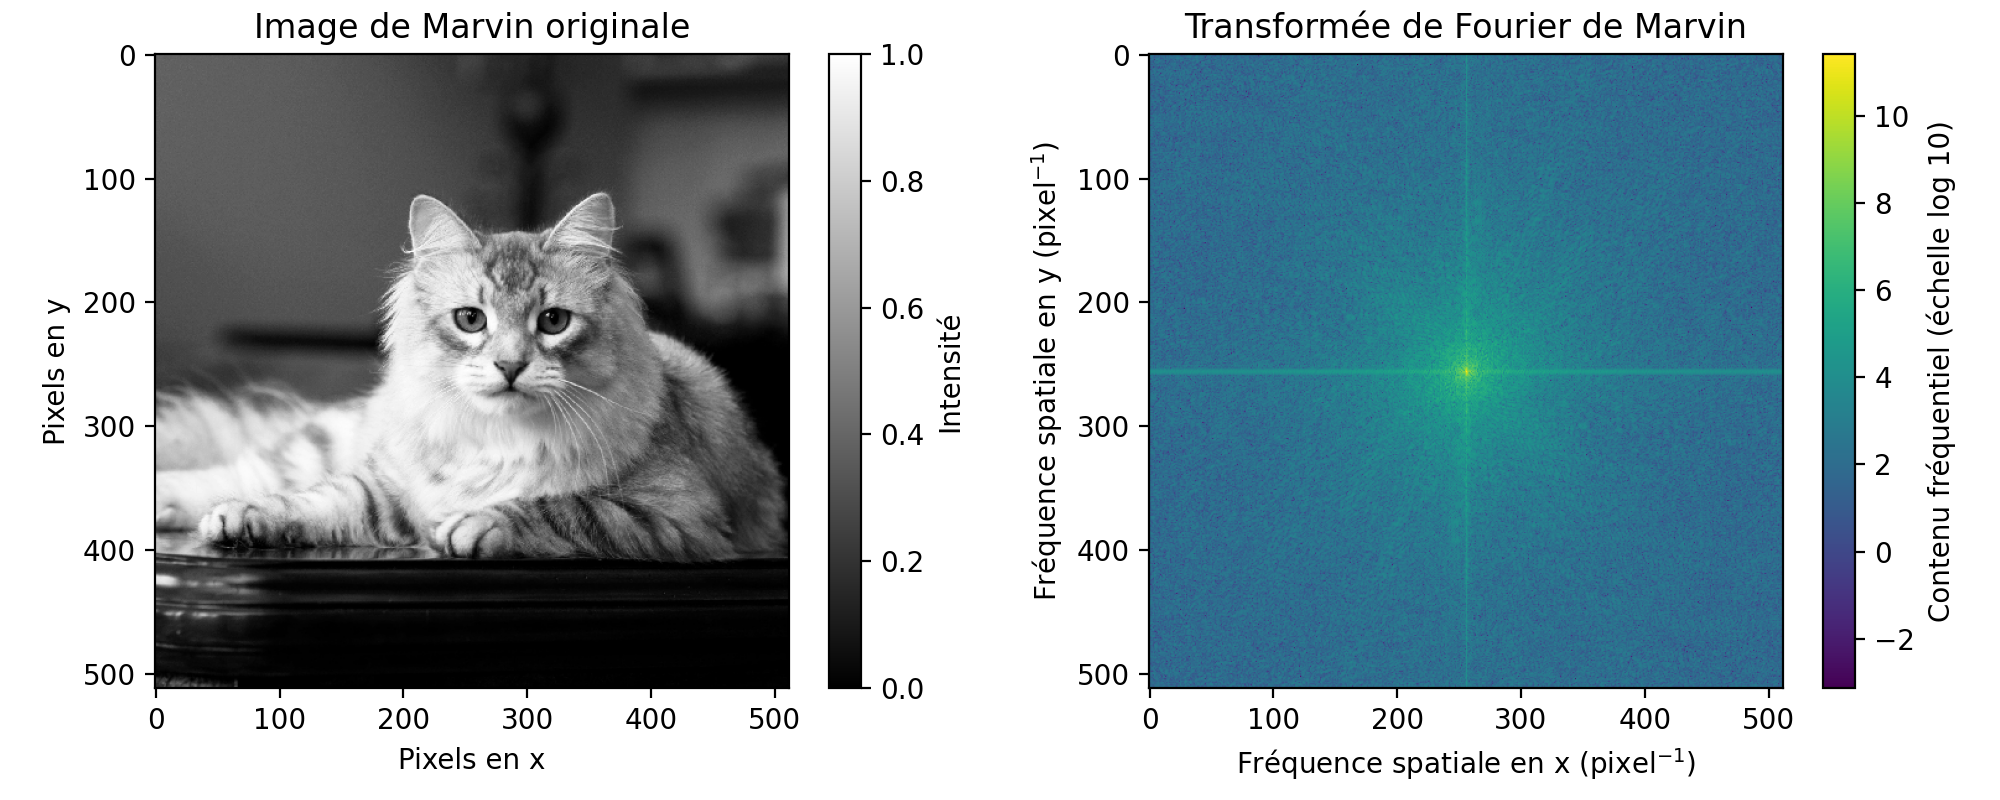
\includegraphics[scale=0.68]{marvin_og.png}
  \caption{Image originale de Marvin et de sa transformée de Fourier}
  \label{cat_og}
\end{figure}

\begin{figure}[H]
  \centering
  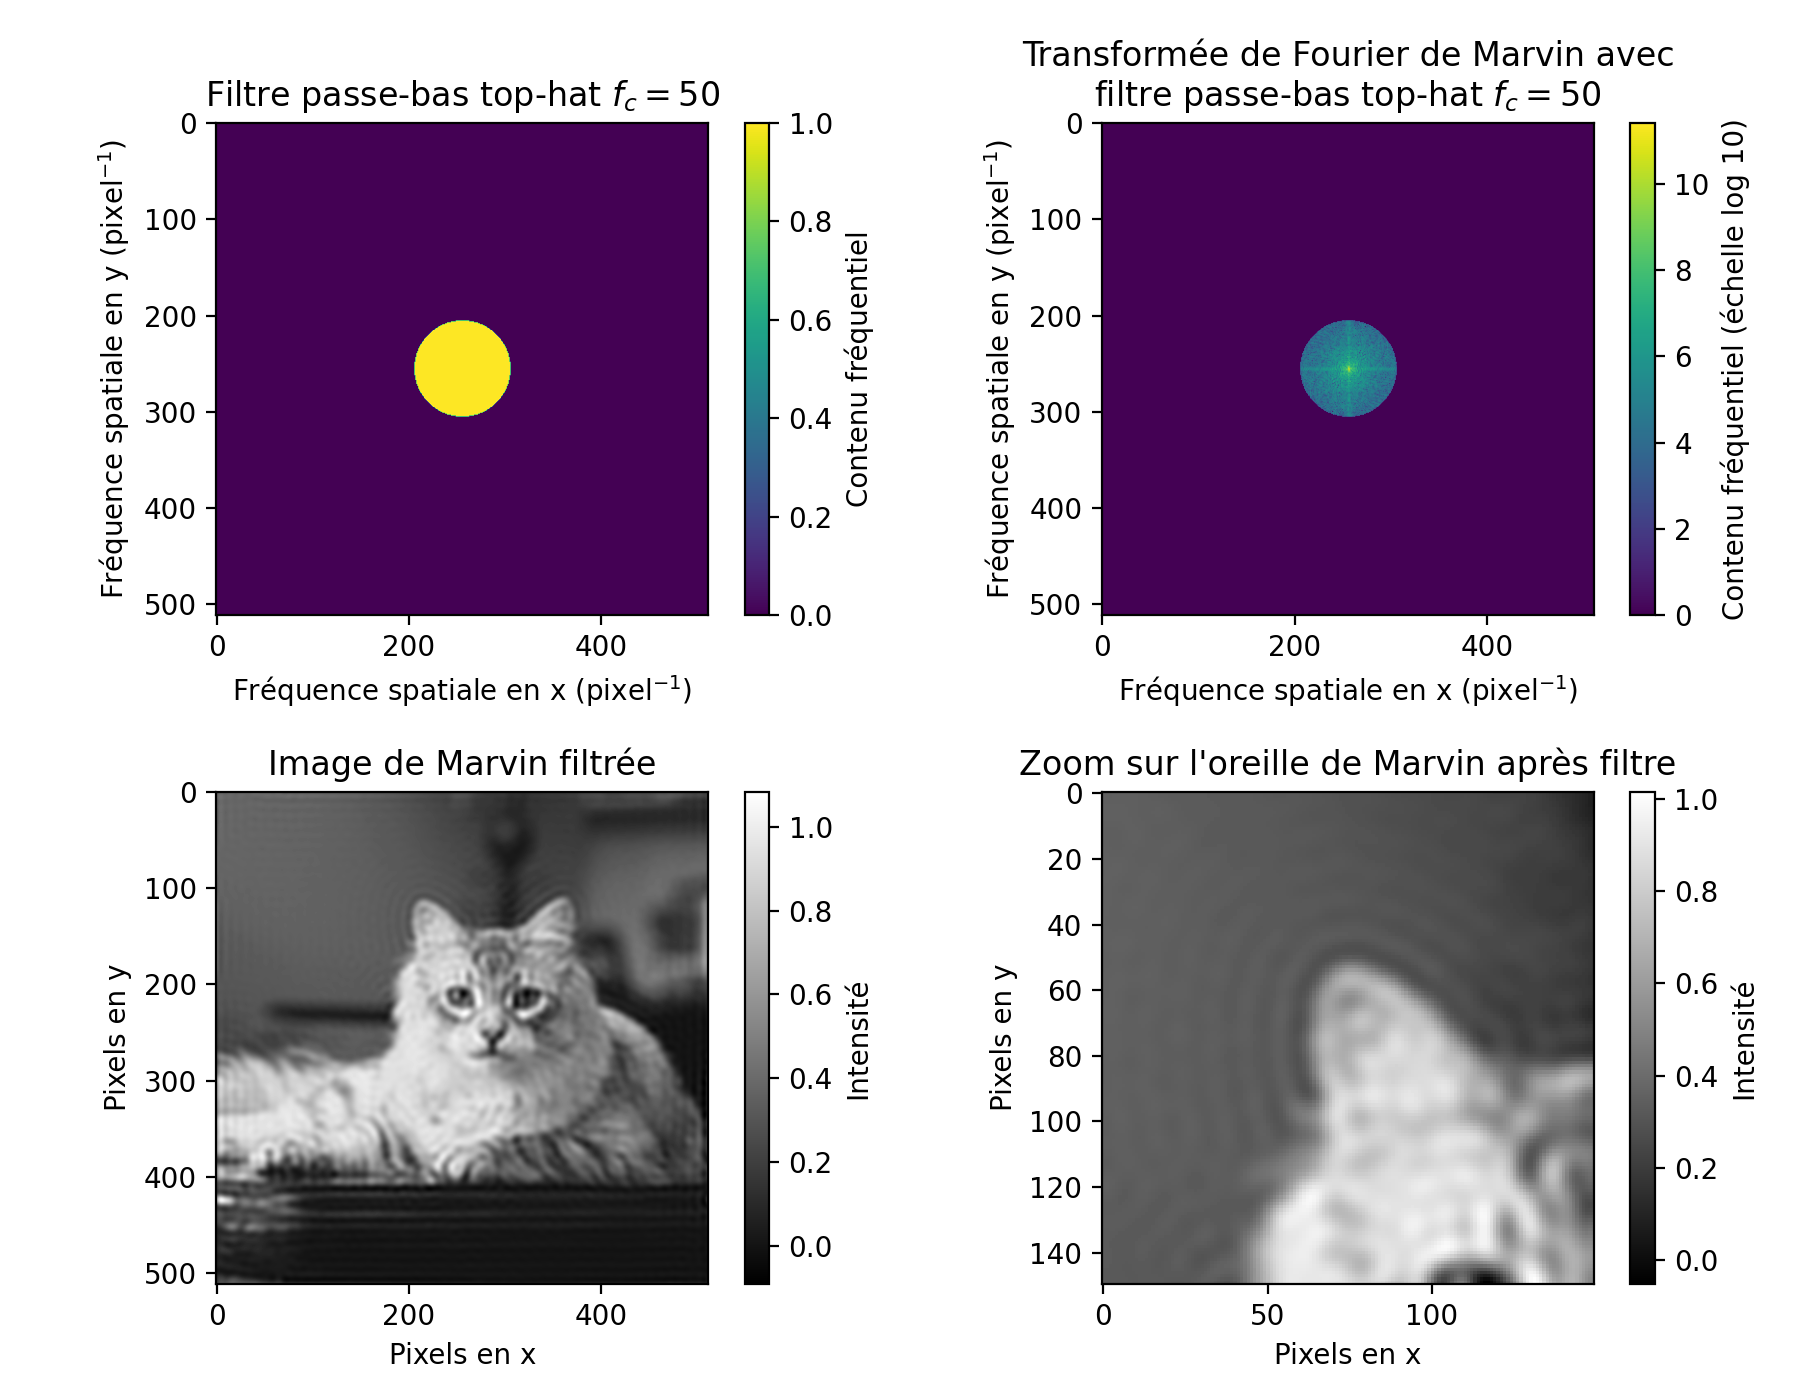
\includegraphics[scale=0.7]{marvin_post_filter_fc_50.png}
  \caption{Filtre passe-bas top-hat à $f_c = 50$ pixels$^{-1}$ appliqué sur l'image de Marvin}
  \label{fc50hat}
\end{figure}

\begin{figure}[H]
  \centering
  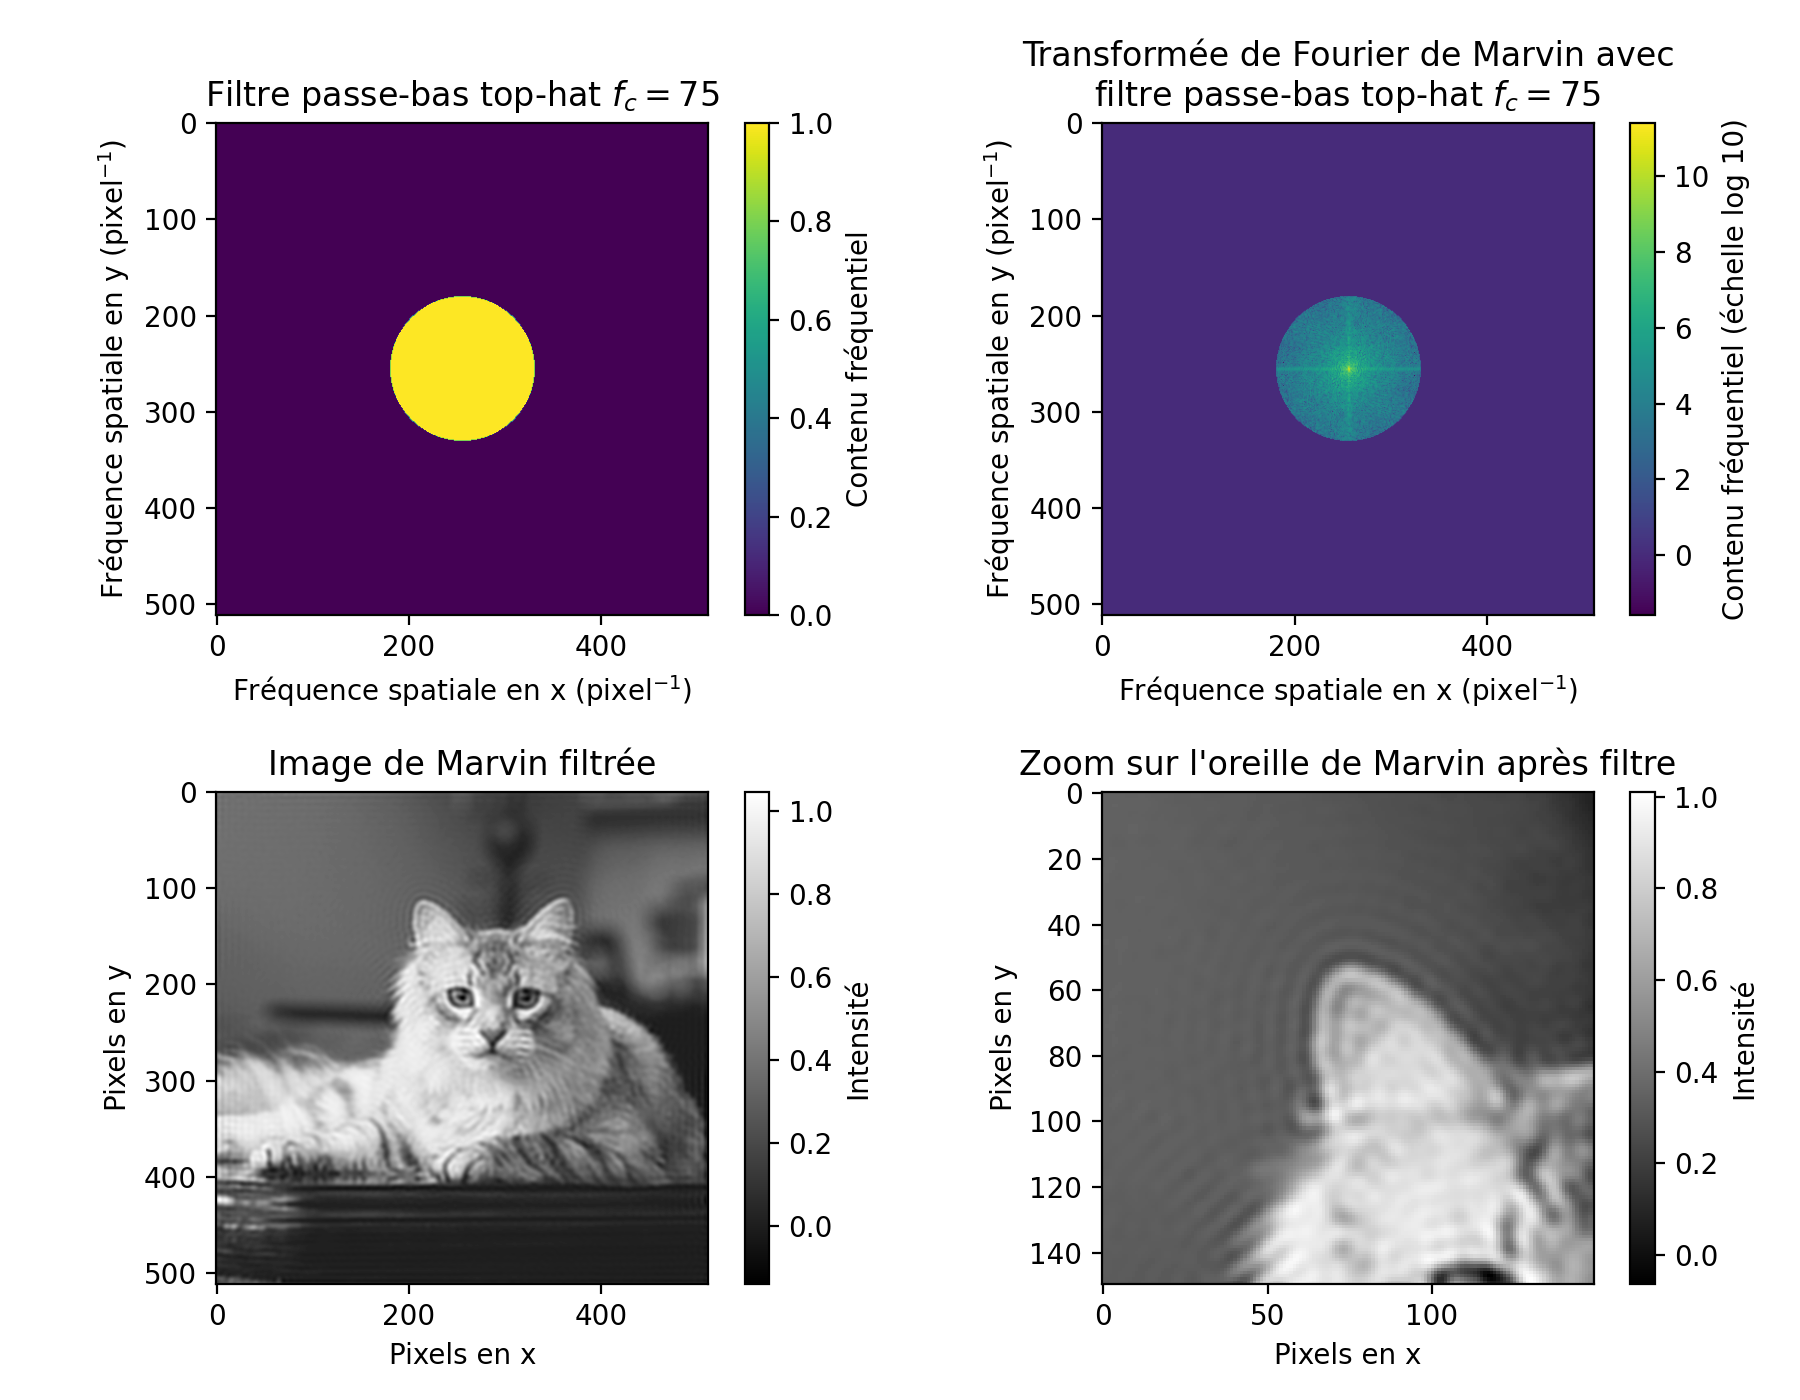
\includegraphics[scale=0.7]{marvin_post_filter_fc_75.png}
  \caption{Filtre passe-bas top-hat à $f_c = 75$ pixels$^{-1}$ appliqué sur l'image de Marvin}
  \label{fc75}
\end{figure}

\begin{figure}[H]
  \centering
  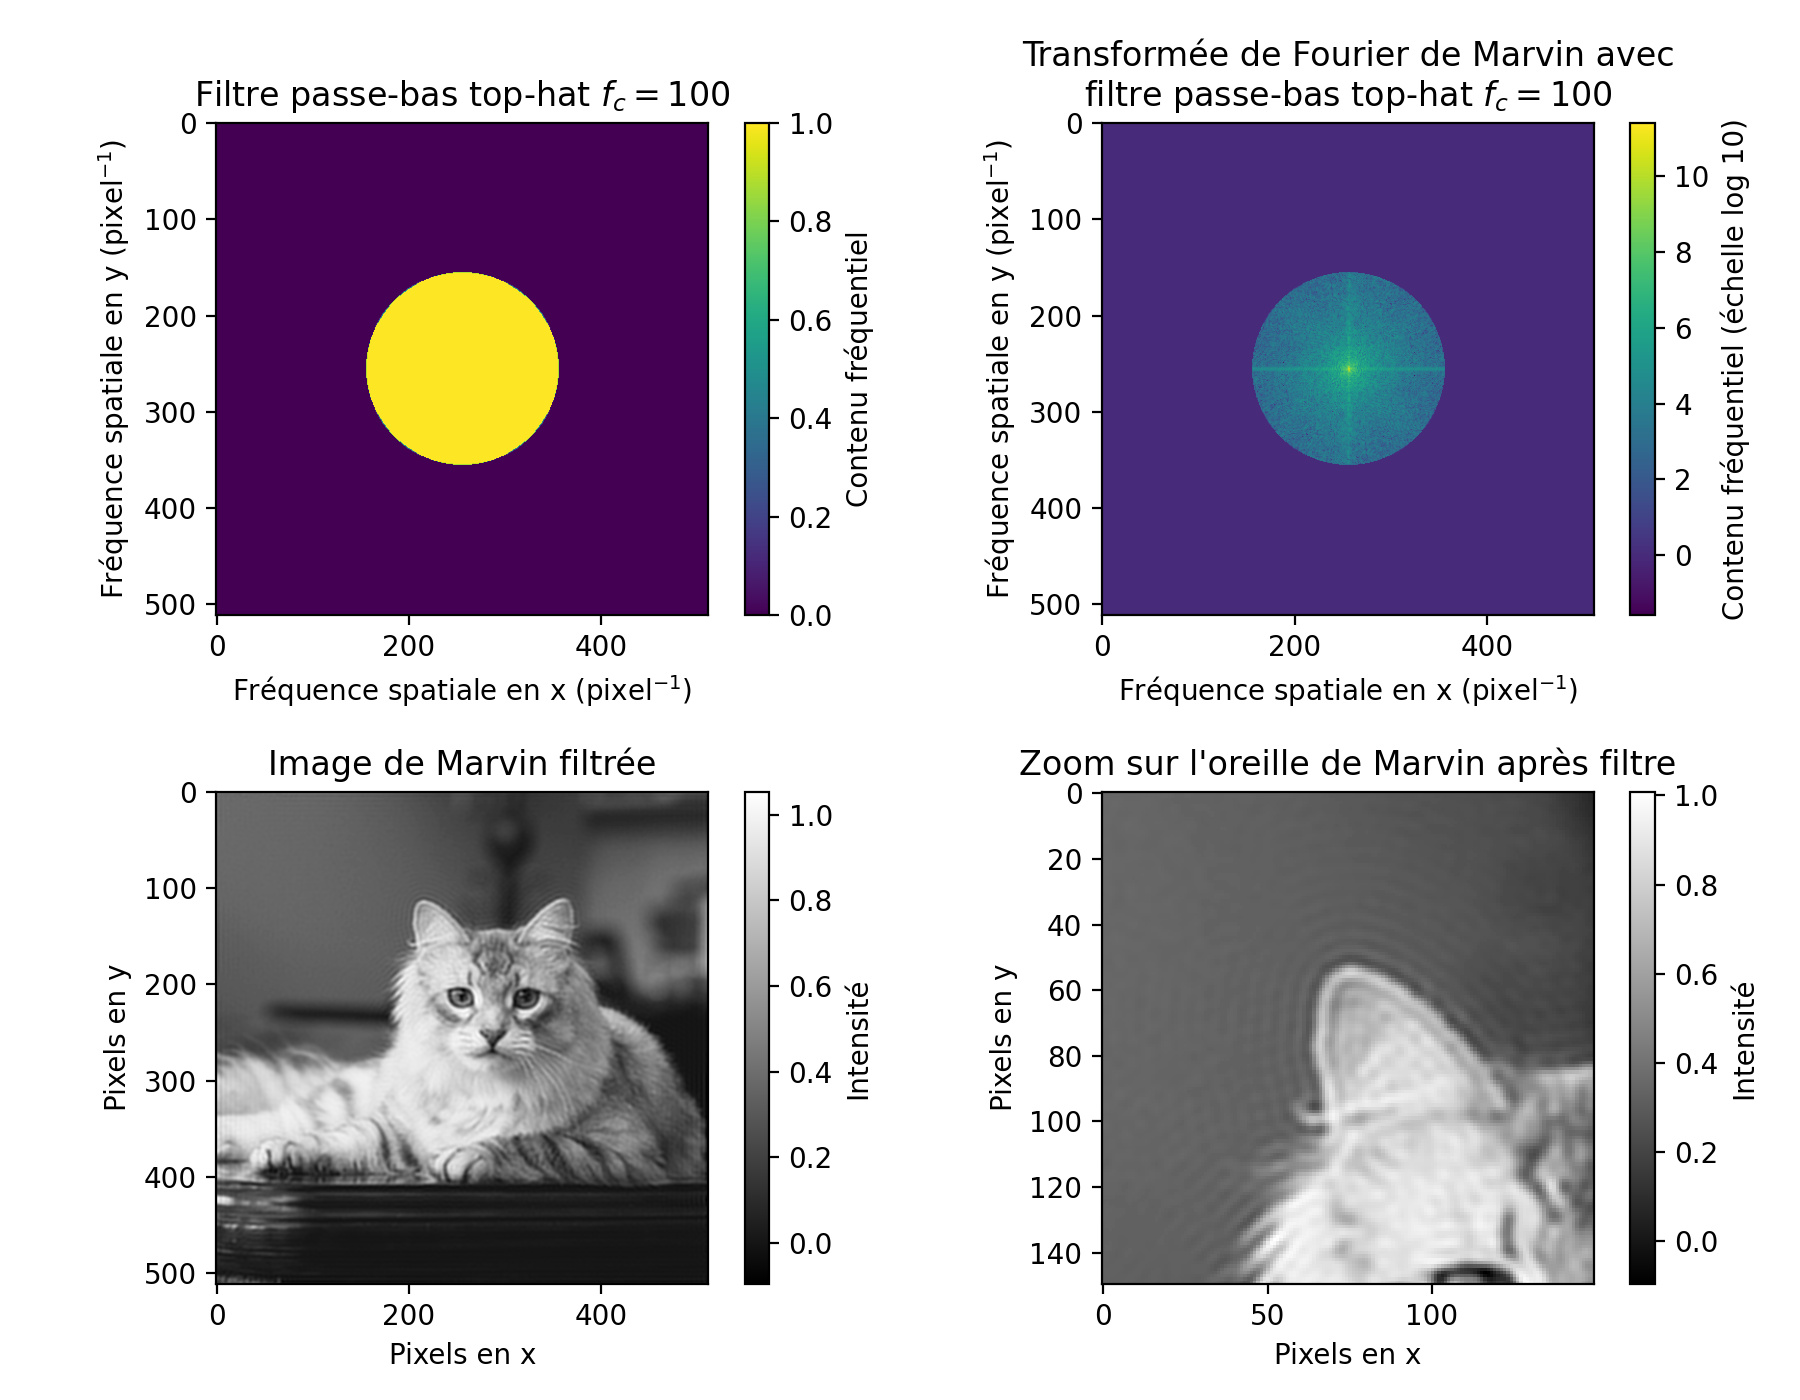
\includegraphics[scale=0.7]{marvin_post_filter_fc_100.png}
  \caption{Filtre passe-bas top-hat à $f_c = 100$ pixels$^{-1}$ appliqué sur l'image de Marvin}
  \label{fc100}
\end{figure}

Pour les trois figures précédentes, un zoom est aussi fait sur l'oreille gauche de Marvin. Il est possible d'y observer une sorte d'onde qui fait le contour de l'oreille et du reste de la tête. Cet effet est plus prononcé pour les filtres de plus basse fréquence. Cela fait en sorte que l'image filtrée la plus claire est celle avec la fréquence de coupure la plus haute, soit $f_c=100$ pixels$^{-1}$ à la figure \ref{fc100}. Il est donc possible d'émettre l'hypothèse que lors des manipulations, la qualité de l'image filtrée augmentera avec l'ouverture de l'iris, qui va agir comme  le filtre passe-bas top hat ici. L'effet ondulatoire sera discuté plus loin.

\subsection{Filtre gaussien}

Enfin, la figure \ref{gauss} montre l'application d'un filtre gaussien, où la fréquence de coupure $f_c = 50$ pixels$^{-1}$ est défini comme l'écart-type de cette gaussienne :

\begin{equation}
  f(x) = e^{\frac{-\left( x-\mu \right)^{2}}{2f_c^2}}
\end{equation}

où $\mu$ est la position au centre de l'image. Cela donne :

\begin{figure}[H]
  \centering
  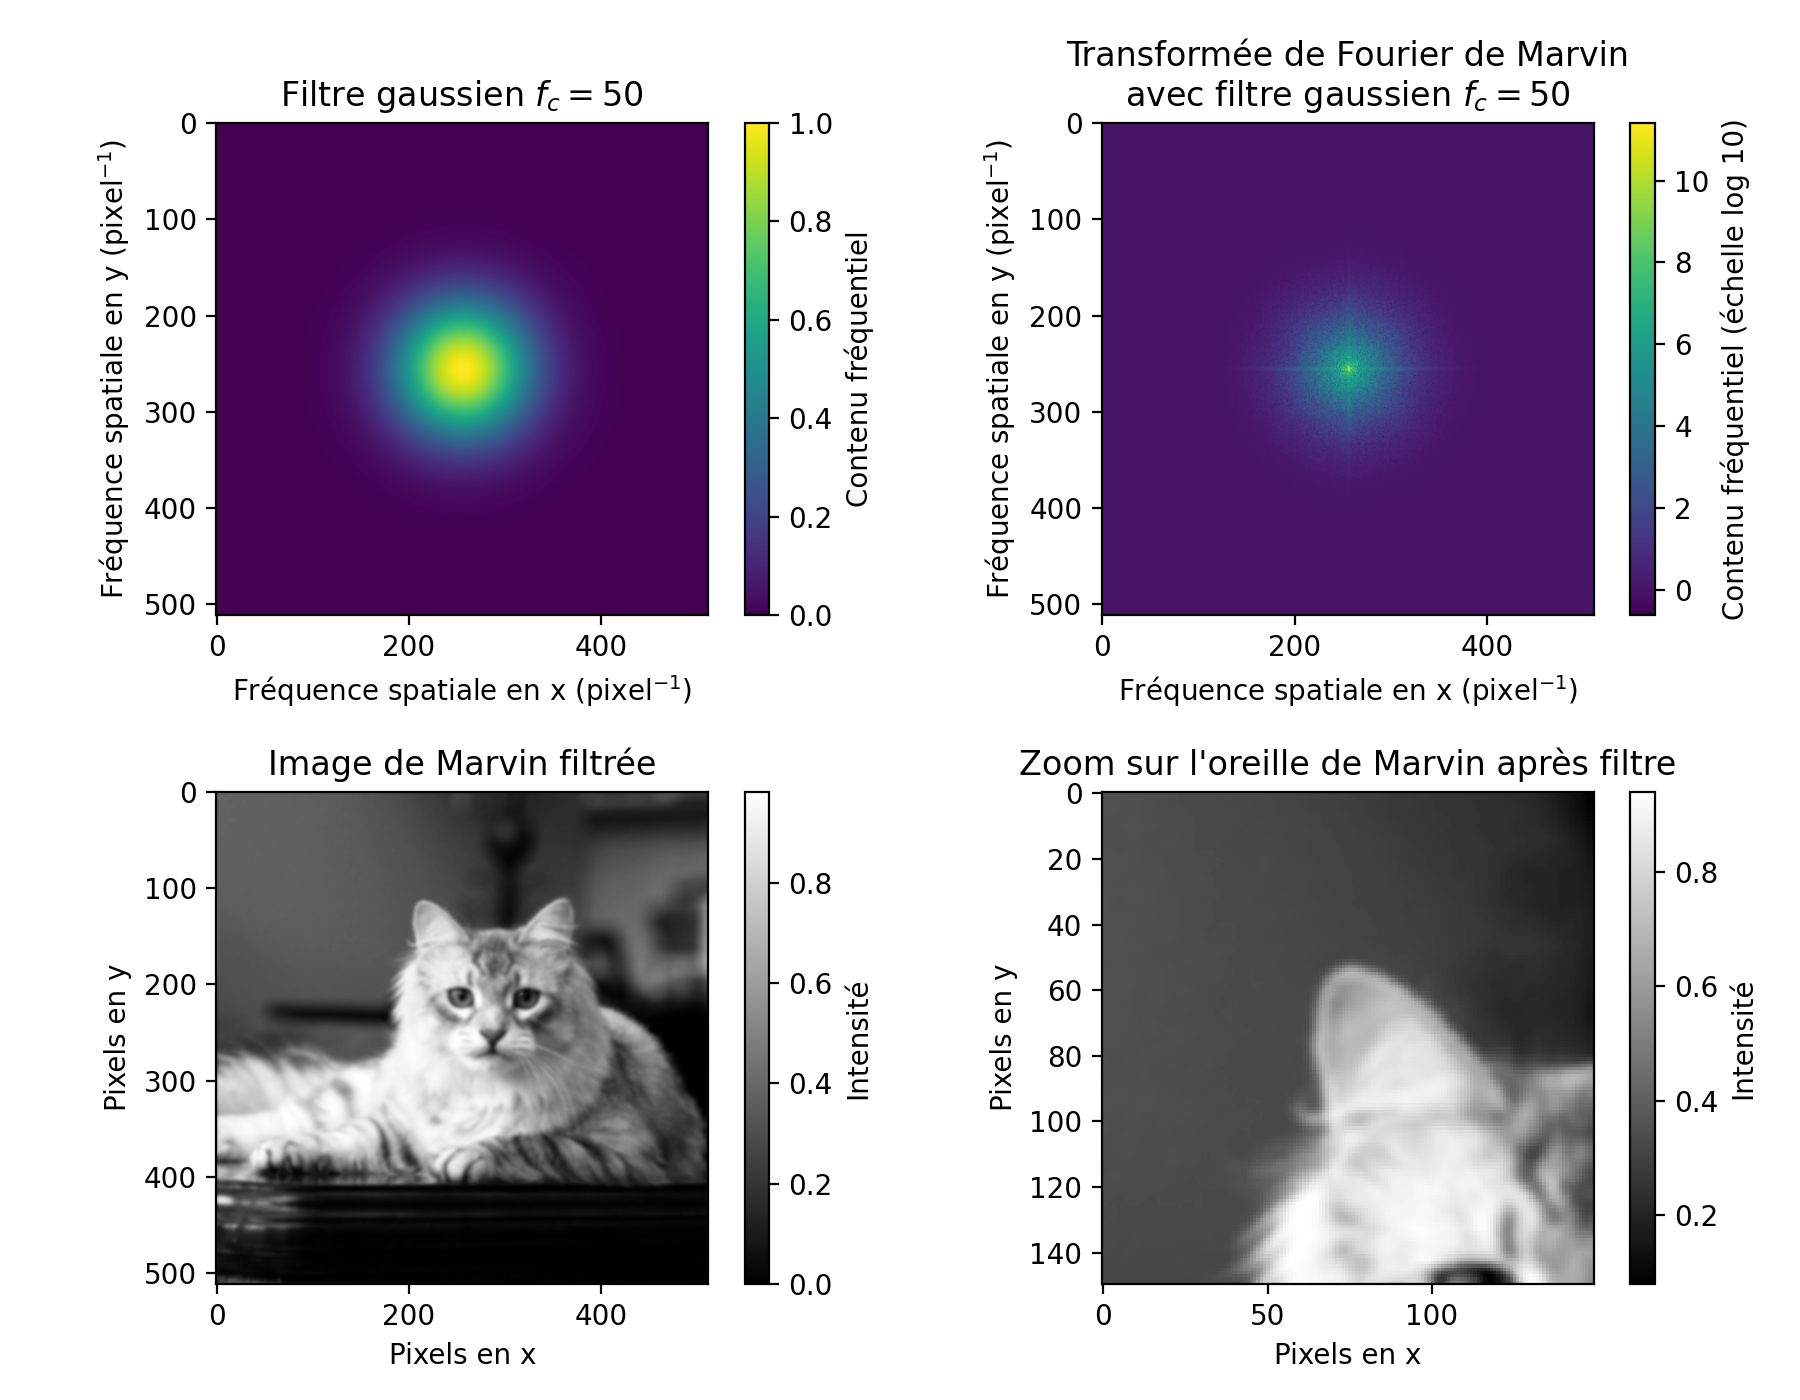
\includegraphics[scale=0.7]{marvin_gauss_fc_50.png}
  \caption{Filtre gaussien à $f_c = 50$ pixels$^{-1}$ appliqué sur l'image de Marvin}
  \label{gauss}
\end{figure}

Le résultat est une image très peu floutée, et en regardant le zoom sur l'oreille, les ondes sont disparues. Le filtre gaussien est donc idéal pour ce cas. Pour expliquer pourquoi le filtre gaussien ne présente pas les ondes, il est bon de se pencher à nouveau sur le filtre top-hat. Ce dernier est essentiellement une fonction rectangle. Sa transformée de fourier est connue comme étant une fonction sinc :

\begin{figure}[H]
  \centering
  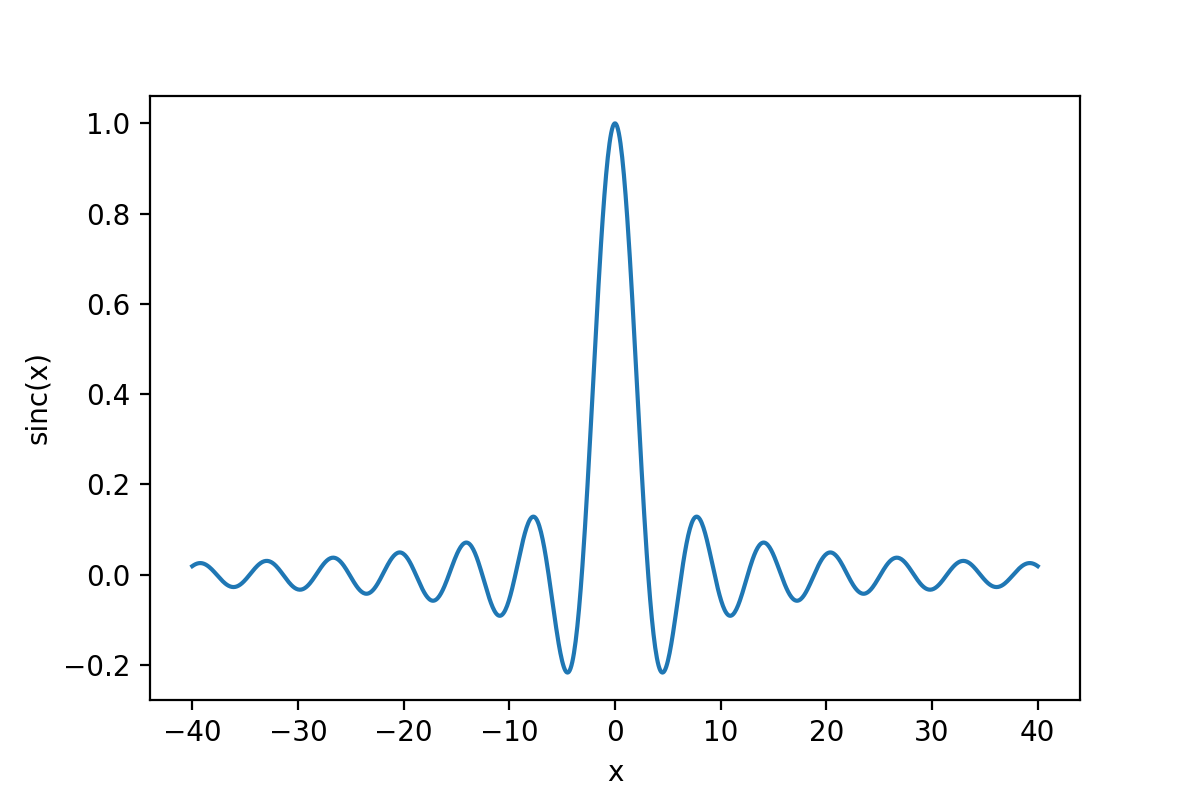
\includegraphics[scale=0.7]{sinc.png}
  \caption{Représentation de la fonction sinc}
  \label{sinc}
\end{figure}

Les ondes observées près des contours sont donc un symptôme de la transformée de Fourier inverse de la fonction rectangle, qui est aussi un sinus cardinal. Les changements drastiques d'intensité voient donc les propriétés du sinc apparaître, notamment les oscillations autour de $\frac{\sin\left( x \right)}{x}  = 0$ pour $x$ éloigné de 0 à la figure \ref{sinc}. C'est l'origine des "ondes" bien visibles près des oreilles de Marvin aux figures \ref{fc50hat}, \ref{fc75} et \ref{fc100}. Quant au filtre gaussien, étant donné qu'une fonction gaussienne est lisse et que sa transformée de Fourier est connue comme étant une autre gaussienne, aucun changement "drastique" ni d'apparence ondulatoire n'est perceptible après le filtrage.

\clearpage

% \bibliographystyle{unsrtnat}
% \bibliography{My_Library}

\end{document}
